\subsection{Frontend}
La modifica dei meeting è disponibile unicamente per le aziende. È possibile:
\begin{itemize}
    \item Modificare data e ora del colloquio.
    \item Aggiungere ulteriori invitati, inserendo le rispettive email.
\end{itemize}
Per poter accedere alla sezione di modifica di un evento, è necessario aprirne i dettagli e cliccare su \textit{"Modifica"}. 
Il \texttt{Dialog} caricato è lo stesso utilizzato per visualizzare i dettagli, sfruttando ancora una volta la renderizzazione
condizionale di React . \cite{reactConditionalRendering}
\begin{figure}[H]   
    \centering
    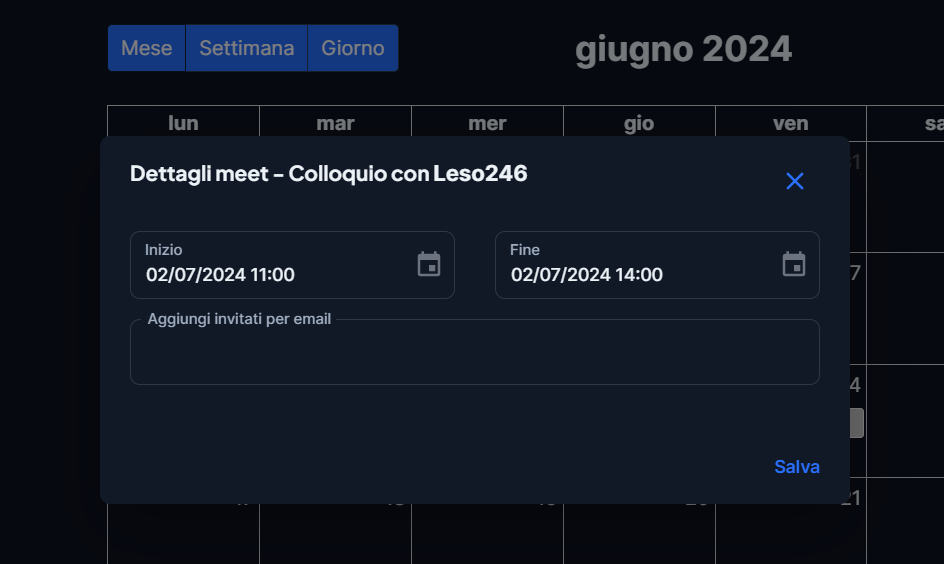
\includegraphics[width=\textwidth]{ModificaMeet/visualizzazioneModifica.png}
    \caption{Visualizzazione Modifica}
\end{figure}
\subsubsection{Modifica di data e ora}
Per cambiare la data e l'ora di un meeting, sono disponibili due modalità: 
\begin{itemize}
    % Sezione dedicata alla scelta dal DateTimePicler
    \item selezionare la data e l'ora dai rispettivi \texttt{DateTimePicker}. Tutte le date passate sono disabilitate e quindi non selezionabili.
    \begin{figure}[H]   
        \centering
        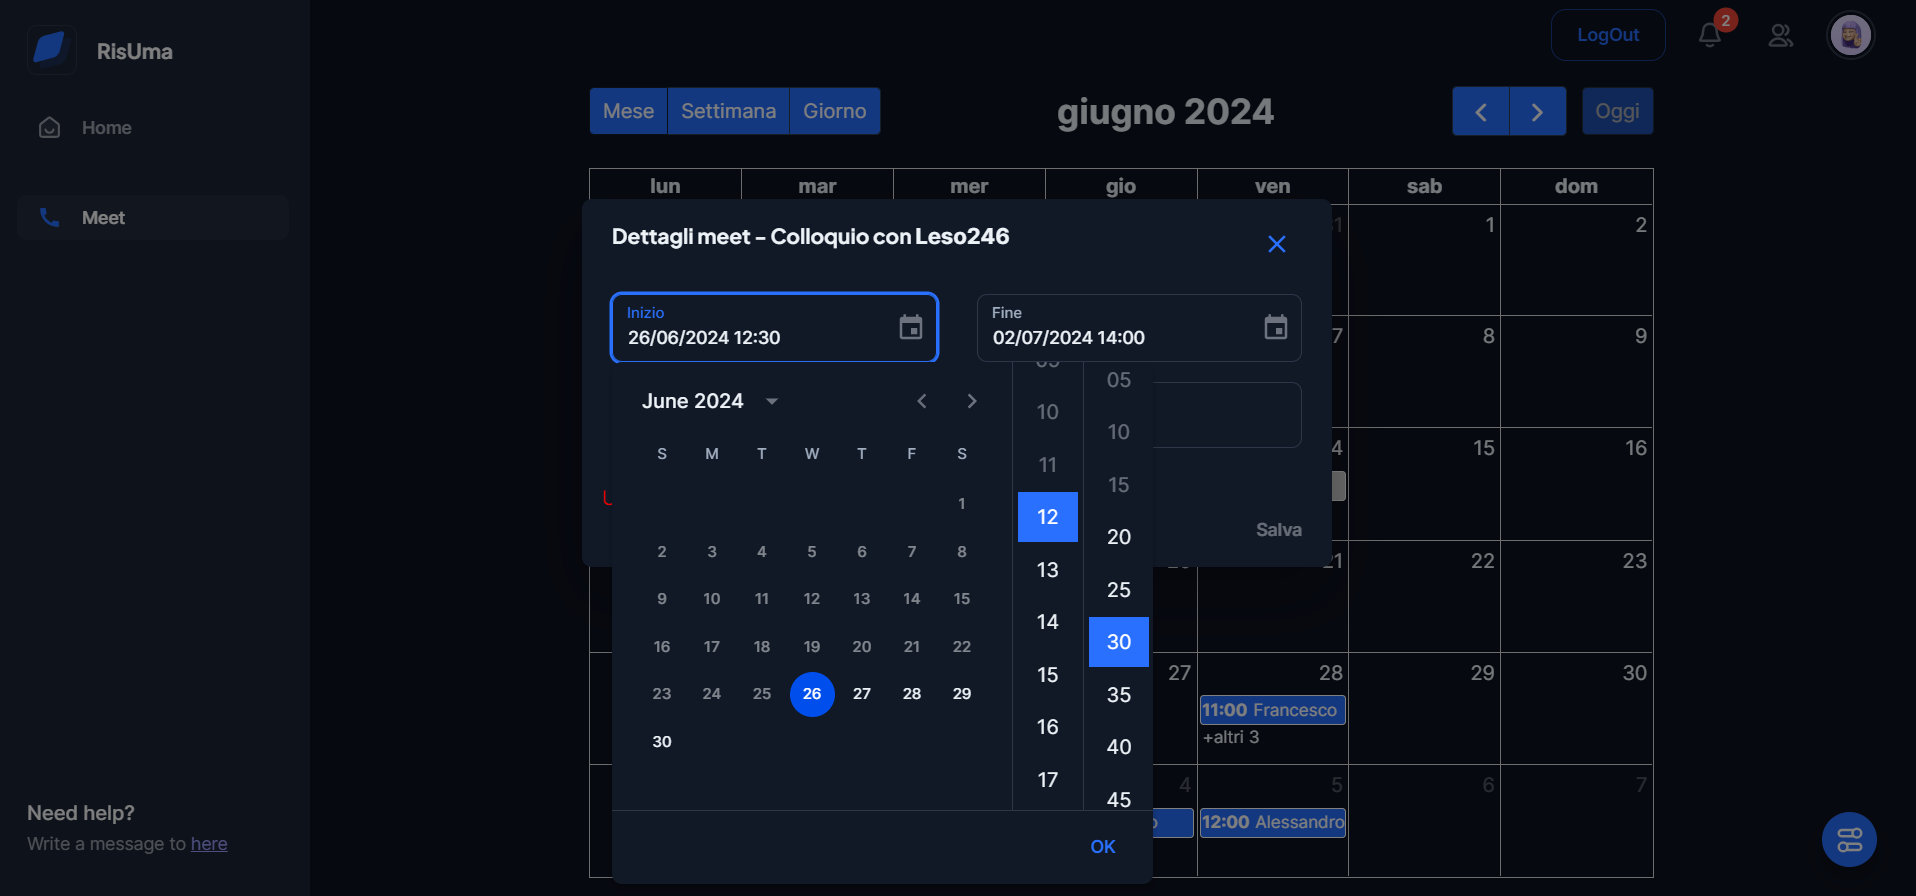
\includegraphics[width=\textwidth]{ModificaMeet/modificaData.png}
        \caption{Modifica di data e ora}
    \end{figure}
    Ci sono tre condizioni da rispettare, le ultime due imposte da Webex: 
        \begin{itemize}
            \item la data di fine non può essere antecedente alla data di inizio.
            \item un meet non può avere una durata inferiore ai 10 minuti.
            \item un meet non può avere una durata superiore alle 24 ore.
        \end{itemize}
    Nel caso si verifichi una di queste tre condizioni, viene visualizzato un messaggio di errore e il pulsante per salvare viene disabilitato.
    \begin{figure}[H]
        \centering
        \begin{minipage}{0.45\textwidth}
            \centering
            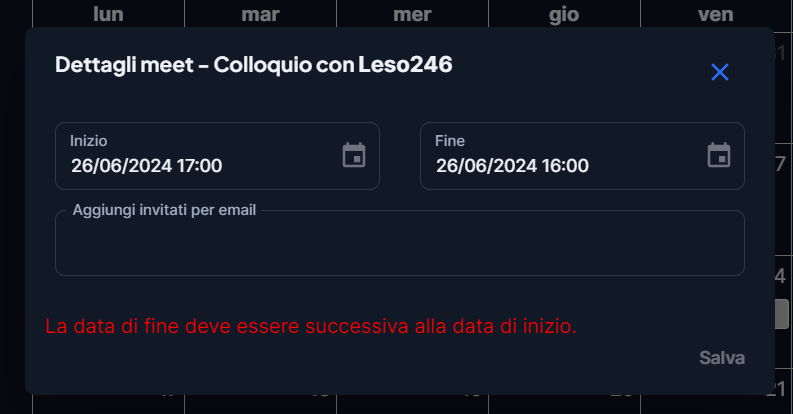
\includegraphics[width=\textwidth]{ModificaMeet/erroreDataFine.png}
            \caption{errore data fine}
        \end{minipage}
        \hspace{0.05\textwidth}
        \begin{minipage}{0.45\textwidth}
            \centering
            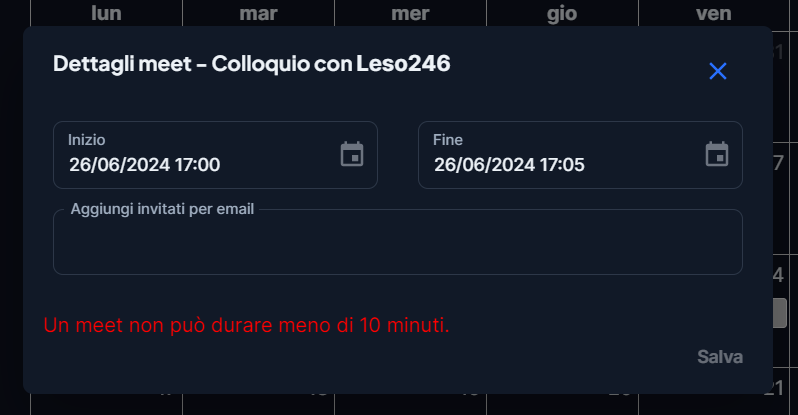
\includegraphics[width=\textwidth]{ModificaMeet/errore10min.png}
            \caption{errore 10 minuti}
        \end{minipage}
        \hspace{0.05\textwidth}
        \begin{minipage}{0.45\textwidth}
            \centering
            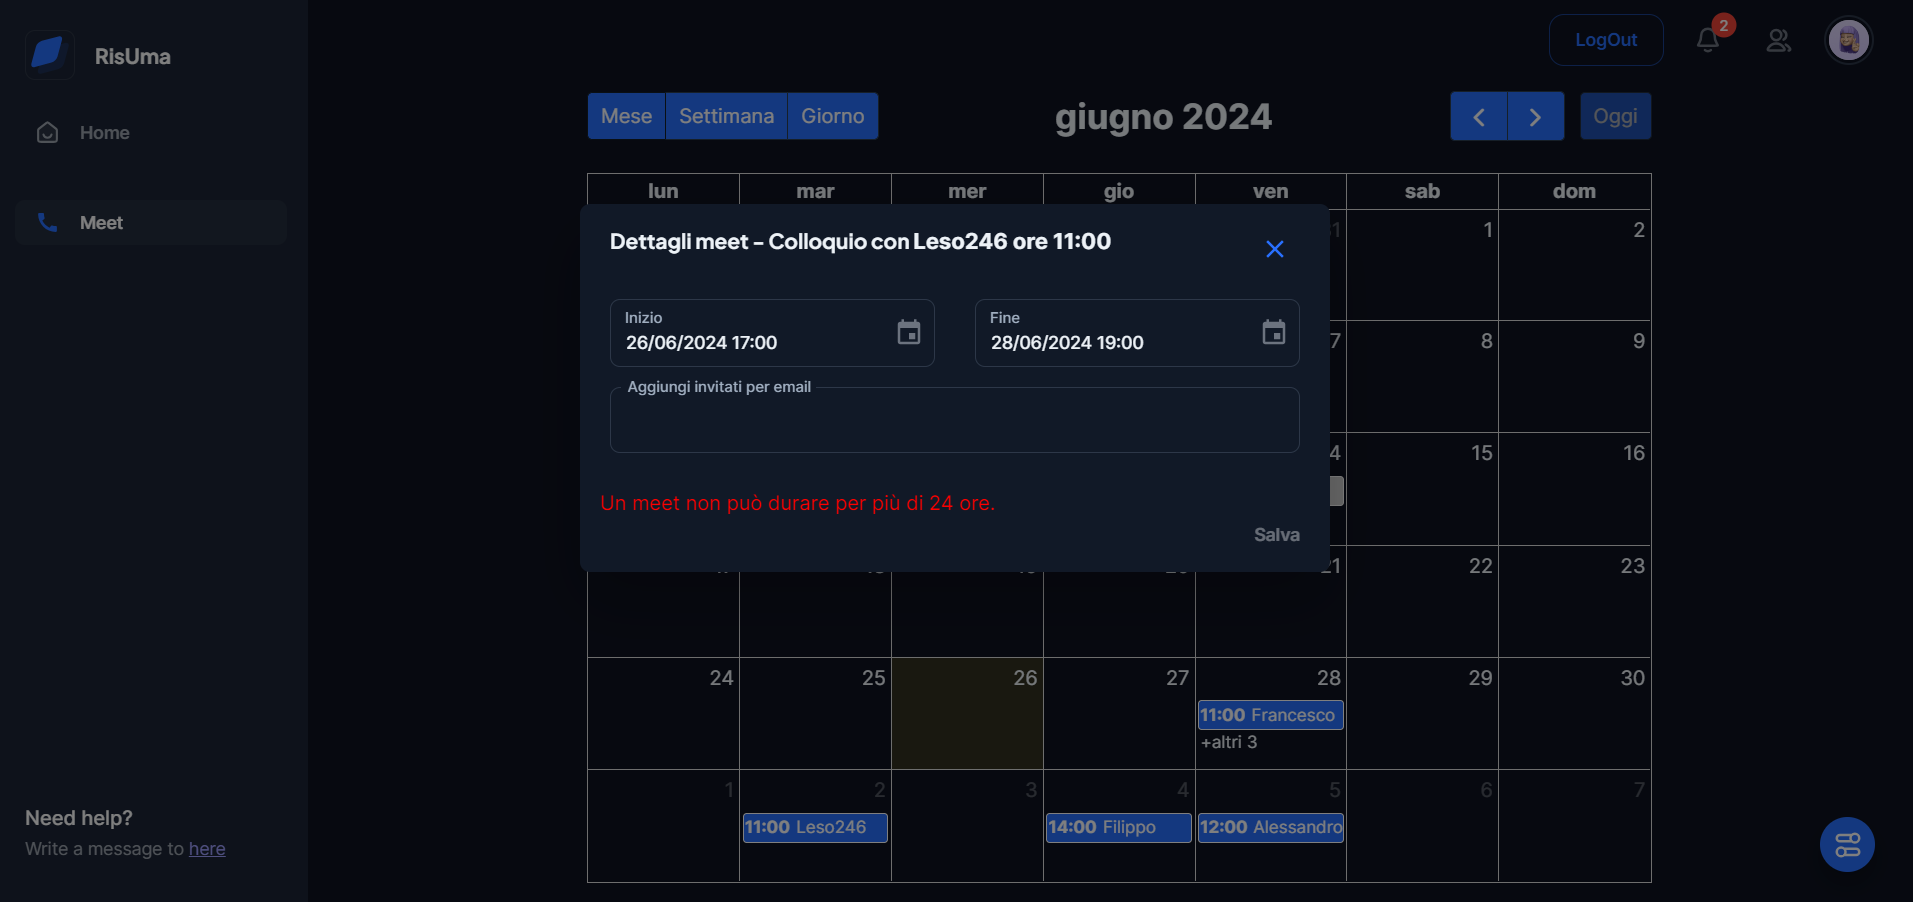
\includegraphics[width=\textwidth]{ModificaMeet/errore24h.png}
            \caption{errore 24 ore}
        \end{minipage}
    \end{figure}
    % Sezione dedicata al drag degli eventi
    \item Trascinando gli eventi a calendario, rilasciandoli sulla data e l'ora desiderate:
        \begin{itemize}
            \item Nella visualizzazione mensile, è possibile cambiare solo la data e non l'ora.
            \item Nella visualizzazione settimanale, è possibile cambiare la data e l'ora con una precisione di mezz'ora rispetto
            all'orario di inizio del meeting.
            \item Nella visualizzazione giornaliera è possibile cambiare unicamente l'ora, sempre con una precisione di mezz'ora.
        \end{itemize}
        \begin{figure}[H]
            \centering
            \begin{minipage}{0.45\textwidth}
                \centering
                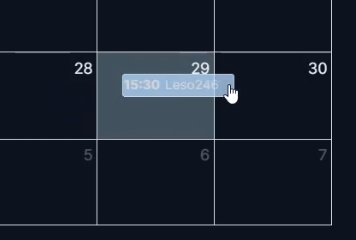
\includegraphics[width=\textwidth]{ModificaMeet/spostamentoEvento.PNG}
                \caption{trascinamento evento}
            \end{minipage}
            \hspace{0.05\textwidth}
            \begin{minipage}{0.45\textwidth}
                \centering
                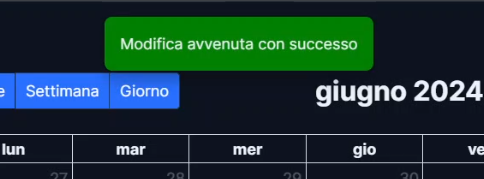
\includegraphics[width=\textwidth]{ModificaMeet/successoModifica.PNG}
                \caption{successo nella modifica}
            \end{minipage}
        \end{figure}
        Nel caso in cui si cerchi di spostare un evento in una data passata, questo viene riportato alla sua posizione originale 
        e l'utente viene avvisato dell'errore tramite un popup.
    \begin{figure}[H]   
        \centering
        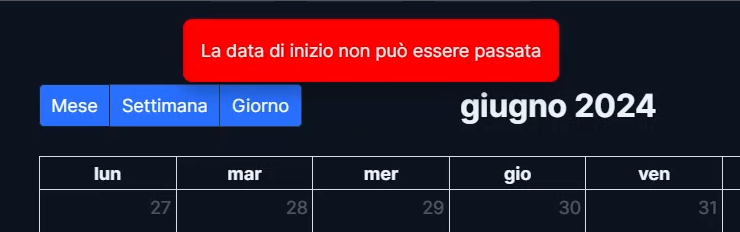
\includegraphics[width=\textwidth]{ModificaMeet/dataInizioPassata.png}
        \caption{Data passata selezionata}
    \end{figure}
    Anche quando viene riscontrato un errore nella modifica, l'utente viene avvisato attraverso un popup e l'evento riportato
    alla posizione originale.
\end{itemize}
\subsubsection{Aggiunta degli invitati}
Per aggiungere invitati a un meet tramite email, è sufficiente digitare gli indirizzi all'interno dell'apposito \texttt{TextField}. 
Quando l'utente inserisce un'email e sposta il focus su un altro elemento, oppure digita uno tra i seguenti caratteri:
\begin{center}
\begin{tabular}{c|c|c|c|c}
Spazio & Invio & , & ; & . \
\end{tabular}
\end{center}
viene effettuato un controllo sull'input digitato. Se l'input viene riconosciuto, attraverso una regex, come un'email valida, 
questa viene visualizzata all'interno di una card per indicare che è stata correttamente riconosciuta e viene contemporaneamente
aggiunta all'array \textit{inviteesList}, uno \texttt{useState}, che verrà inviato al backend.
\begin{figure}[H]
\centering
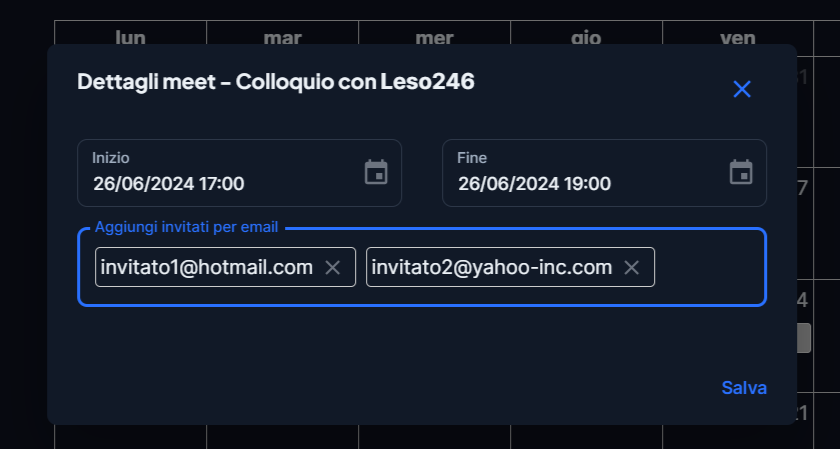
\includegraphics[width=\textwidth]{ModificaMeet/AggiungiInvitati.png}
\caption{Aggiunta degli invitati}
\end{figure}
\noindent Se si desidera modificare un'email, basta cliccarci sopra per ritornare alla visualizzazione del testo. 
Per eliminarla, è possibile cliccare sulla \textit{X}. 
\\
Sorge un problema: se l'utente digita una sola email e, senza spostare il focus dal \texttt{TextField}, 
clicca sul pulsante \textit{Salva}, l'email digitata non sarà aggiunta come card e quindi non sarà inclusa nell'array
di email da inviare al backend. Per tale motivo, al momento del salvataggio, è necessario controllare l'input 
rimasto all'interno del \texttt{TextField} e, se questo risulta essere un'email valida, aggiungerla all'array di invitati.
\subsubsection{Salvataggio delle modifiche}
Quando si salvano le modifiche, viene chiamata la funzione \texttt{modifyMeet}:
\begin{lstlisting}[language=typescript, frame=lines, basicstyle=\ttfamily\scriptsize, numbers=left]
const modifyMeet = async () => {

    const payload = {
        evento: isDragged ? modifiedDraggedEvent : eventDetails,
        invitati: inviteesList,
    };

    try {
        const response = await modifyMeeting(payload);
        if (response.status == 200) {
            showPopup('Modifica avvenuta con successo', true);
            
            if (!isDragged) {
                const updatedEvents = events.map((event) =>
                event.id == eventDetails.id ? { ...event, ...eventDetails } : event
            );
            setEvents(updatedEvents);
            }
        } else
...
\end{lstlisting}
\begin{itemize}
    \item \textbf{Righe 3-6}: viene costruito l'oggetto da inviare a backend. Questo include il JSON dell'evento modificato e l'array
    di stringhe contenente le email da aggiungere agli invitati. \texttt{isDragged} è un \texttt{boolean} che indica se l'evento
    è stato modificato dall'intrefaccia del \texttt{Dialog} o se è stato trascinato, in base al suo valore viene passato 
    l'evento corretto.
    
    \item \textbf{Righe 13-17}: se l'operazione di modifica dell'evento dall'interfaccia del \texttt{Dialog} ha
    avuto successo, gli eventi del \texttt{Fullcalendar} vengono aggiornati manualmente in modo da visualizzare la modifica senza che 
    si debba ricaricare la pagina.
\end{itemize}
Inoltre, tutte le persone invitate al meeting ricevono una email di notifica riguardante la modifica apportata.